\documentclass{article}
\usepackage{enumerate}
\usepackage[a4paper, margin=.5in]{geometry}
\usepackage[table]{xcolor}
\usepackage{graphicx}
\graphicspath{ {./images/} }

\title{Submission 2.1}
% \author{Saffron Liu}
\date{}
\begin{document}
\maketitle

\begin{enumerate}
      \item Translate into smooth English: $\forall x\forall y((Px \land Ty \land Dxy \land Oxy) \to \neg \exists z(Pz \land Kzxy))$.\\
            Let “Px” mean “x is a person”, “Tx” mean “x is a time”, “Dxy” mean “x is down at time y”, “Oxy” mean “x is out at time y”, and “Kxyz” mean “x knows y at time z”.\\
            Every pair of individuals x and y is such that if x is a person, y is a time, x is down at time y, and x is out at time y, then there is no z such that if z is a person, z knows x at time y. More English-y: If someone is down and out, they cannot be known by someone else at that time. Even more English-y: Nobody knows you when you're down and out.
\end{enumerate}

\begin{flushleft}
      For problems 2-15: \textit{Write a sentence in quantificational logic that captures as much of the given information as possible. Remember to delineate the extensions you assign to names and predicates.}
\end{flushleft}
\begin{enumerate}
      \setcounter{enumi}{1}
      \item All's well that ends well. (Shakespeare) (B 148)\\
            Ax: x is well\\
            Bx: x ends well\\
            $\forall x(Bx \to Ax)$
      \item The things which are seen are temporal; but the things which are not seen are eternal. (II Corinthians 4:18) (B 169)\\
            Ax: x is seen\\
            Bx: x is eternal\\
            $\forall x((Ax \to \neg Bx) \land (\neg Ax \to Bx))$, which is equivalent to $\forall x (Ax \leftrightarrow \neg Bx)$.
      \item 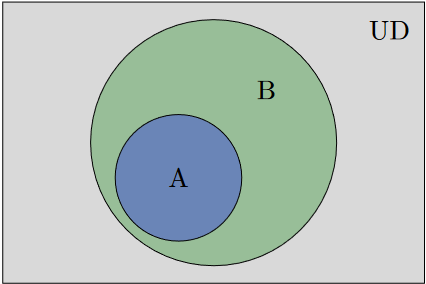
\includegraphics{2.1.4} \\
            Ax: x is in A\\
            Bx: x is in B\\
            $\forall x(Ax \to Bx)$
      \item 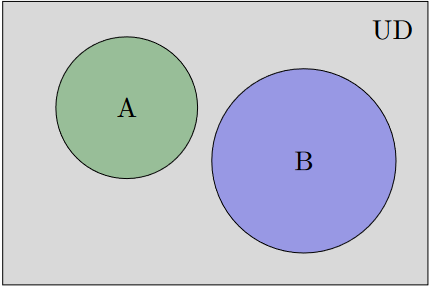
\includegraphics{2.1.5}\\
            Ax: x is in A\\
            Bx: x is in B\\
            $\forall x(Ax \leftrightarrow \neg Bx)$
      \item If you don't love yourself, you can't love anybody else.\\
            Lxy: x loves y\\
            y: you\\
            $\neg Lyy \to \neg \exists x(Lyx)$
      \item NSYNC is the best band ever.\\
            n: NSYNC\\
            A: is the best band\\
            $An$
      \item Somebody loves everybody.\\
            Axy: x loves y\\
            $\exists x \forall y (Axy)$
      \item There is someone for everybody.\\
            Axy: There is x for y\\
            $\forall y \exists x(Axy)$\\
            \textit{Note: the order of quantifiers matters!}
      \item Scrooge doesn't love anybody.\\
            Axy: x loves y\\
            s: Scrooge\\
            $\neg \exists x (Lsx)$
      \item Only the shallow know themselves. (Oscar Wilde) (B 169)\\
            Ax: x is shallow\\
            Bx: x knows itself\\
            $\forall x(Bx \to Ax)$
      \item Everybody has a mother.\\
            Ax: x has a mother\\
            $\forall x(Ax)$
      \item There are at least two pigs.\\
            Px: x is a pig\\
            $\exists x \exists y (Px \land Py \land (x \neq y))$
      \item There are exactly two pigs.\\
            $\exists x \exists y \exists z (Px \land Py \land x \neq y \land ((z \neq x \land z \neq y) \to \neg Pz))$
      \item There are at most two pigs.\\ 
            $\neg \exists x \exists y \exists z (Px \land Py \land Pz \land (x \neq y \land x \neq z \land y \neq z))$
            \textit{(there are not 3 unique pigs)}
      
\end{enumerate}

\end{document}